\section{Experiments}\label{sec:experiments}
We compute the constants of Sections~\ref{sec:general}--\ref{sec:model} for trained rules and check them in simulated audits. Every population $P$ is a held-out or target empirical law mixed with a uniform mass of $1\%$ over profiles and labels, which gives full support; every design-based score is pointwise unbiased; and every constant is certified by primal and dual bounds that agree to a relative error of at most $10^{-4}$ ($10^{-3}$ within a model) unless a bound or an interval is shown. Ratios are between the best designs of two classes at $P$. Protocols, per-run values and sensitivity analyses are in Appendix~\ref{app:F}.

\begin{table*}[t]
\centering
\caption{BRFSS screening trees on twelve items (six runs per cap: two targets, three seeds): records that pre-committed forms need relative to branching interviews; medians over runs, range in brackets. \emph{Without a model} (design-unbiased scores; branching asks the tree\textquotesingle s own questions and attains the full-information variance): Oracle, optimal forms at the target law; Reference, forms fitted on 20,000 source records; Pilot, forms learned from a pilot of a quarter of $N=4{,}000$ audit records smoothed by a pairwise fit, pilot charged (runs with a gain); U-paths, uniform over the tree\textquotesingle s question paths with the best scores; Two rounds, optimal two-round design (at $b=6$ the median includes certified upper bounds from feasible two-round designs for 4 runs, Table~\ref{tab:runs}); Bracket, the ends $1/\rho_P^2$ and $N_P$ of Theorem~\ref{thm:bracket}. \emph{Within a model}: $W^{(k)}_{\rm fixed}/W^{(k)}_{\rm branch}$ at the order-$k$ log-linear fit of the target law, with every class at its optimum (one for runs whose rule depends on at most $b$ items; at $b=6$, $k=3$ the branching optimum is bracketed to within \nModelGapSix\%, so the ratios are lower bounds). On thyroid (24 runs) every optimized ratio is $1.00$. -- not computed.}
\label{tab:screening}
\footnotesize
\setlength{\tabcolsep}{5pt}
\begin{tabular}{r l r r r r l l l}
\toprule
 & \multicolumn{6}{c}{without a model} & \multicolumn{2}{c}{within a model} \\
\cmidrule(lr){2-7}\cmidrule(lr){8-9}
$b$ & Oracle & Reference & Pilot & U-paths & Two rounds & Bracket & pairwise ($k=2$) & three-way ($k=3$) \\
\midrule
3 & 1.00 [1.00, 1.34] & 1.04 & -- & 1.03 & 1.00 & [1.00, 1.5] & 1.00 [1.00, 1.09] & 1.00 [1.00, 1.23] \\
4 & 1.49 [1.00, 1.75] & 1.57 & 1.65 & 1.80 & 1.00 & [1.18, 3.3] & 1.09 [1.00, 1.13] & 1.28 [1.00, 1.40] \\
5 & 1.35 [1.18, 1.54] & 1.42 & 1.53 & 1.72 & 1.00 & [1.08, 5.4] & 1.06 [1.02, 1.10] & 1.17 [1.08, 1.28] \\
6 & 1.58 [1.42, 1.98] & 1.68 & 1.93 & 2.30 & $\le$1.05 & [1.13, 10.5] & 1.07 [1.05, 1.13] & $\ge$1.18 [1.15, 1.33] \\
\bottomrule
\end{tabular}
\end{table*}


\paragraph{Screening questionnaires.}
A depth-$b$ screening tree asks at most $b$ questions per person, so a validation study under the same burden must respect the cap. We train class-balanced CART trees on twelve yes/no items of the CDC Diabetes Health Indicators, derived from the Behavioral Risk Factor Surveillance System (BRFSS; 253,680 respondents, target diabetes or prediabetes) \citep{cdcdiabetes2017}, and on twelve binarized thyroid items (7,200 patients) \citep{quinlan1986thyroid}, and validate them on a disjoint random half or on respondents of the other sex (Tables~\ref{tab:screening} and~\ref{tab:runs}). On thyroid, and for the BRFSS trees that use at most $b$ items, one form asks everything the rule needs and pre-commitment costs nothing.

\emph{Without a model.} On BRFSS at caps four to six the best pre-committed design needs a median \nScreenBestLo--\nScreenBestHi{} times the respondents of branching (\nScreenRunLo--\nScreenRunHi{} over runs); label-dependent form probabilities lower this by at most \nLabelMax\%. These are oracle designs. Forms fitted on 20,000 source records need a median \nFitMed\% more and stay exactly unbiased. With no reference, the design is learned from a pilot of the audit itself, which must be charged: with a quarter of $N=4{,}000$ records as a cross-fitted pilot on the tree's paths and cell masses smoothed by a pairwise fit, the all-in price is \nSmoothFourc, \nSmoothFivec{} and \nSmoothSixc{} at $b=4,5,6$, against \nSmoothFourBest, \nSmoothFiveBest{} and \nSmoothSixBest{} for the oracle; unsmoothed pilot frequencies give \nSmoothEmpFourc, \nSmoothEmpFivec{} and \nSmoothEmpSixc{} (Table~\ref{tab:pilotsmooth}). Optimization matters: uniform randomization over the tree's own question paths needs a median \nUpsOverMed\% more records than the optimized design, and uniform matrix sampling over all forms \nUnifLo--\nUnifHi{} times the records of branching. A second round removes most of the gap: \nGainComputable{} of the \nScreenGainN{} BRFSS trees with a gain are computed exactly by a two-round interview, \nGainExactNon{} more have an optimal two-round design within a factor \nScreenTwoMax{} of branching, and for the remaining \nTwoBounded, at $b=6$, feasible designs found in an hour are within \nTwoBoundMax. The bracket of Theorem~\ref{thm:bracket} is loose here: its lower end is a median factor \nLowUnder{} below the realized ratio and its upper end \nNpOver{} above, so the solver is needed.

\emph{Within a model.} We refit each target law by the pairwise and the three-way log-linear model on the label and the rule's items and compute $W^{(k)}$ for forms and for depth-$b$ trees at the fit (\nModelRuns{} runs in which the rule depends on more than $b$ items; Table~\ref{tab:model}). Under the pairwise model pre-committed forms need \nModelTwoLo--\nModelTwoHi{} times the records of the best branching design, where the design-based ratio at the same laws is \nModelDesignLo--\nModelDesignHi: the model removes a median \nModelTwoRemoved\% of the log-gap. Both classes also need fewer records than design-based branching, \nModelTwoFixLo--\nModelTwoFixHi{} and \nModelTwoBrLo--\nModelTwoBrHi{} of its constant. Under the three-way model the ratio is \nModelThreeLo--\nModelThreeHi. The pattern of Theorem~\ref{thm:structured}(c) thus holds on real populations: the less interaction the analyst allows, the less adaptivity is worth.

\begin{figure}[t]
\centering
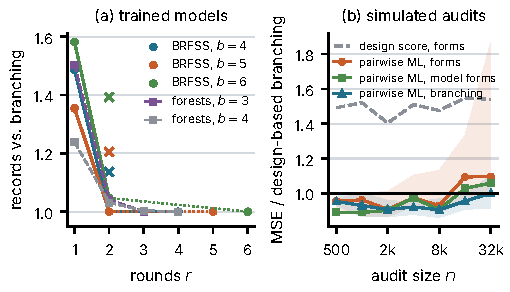
\includegraphics[width=\columnwidth]{figures/v17_rounds.pdf}
\caption{(a) Records needed relative to branching, without a model, as a function of the number of rounds ($r=1$: fixed forms; $r=b$: branching): optimal $r$-round designs for BRFSS screening trees (median over runs; at $b=6$, $r=2$ the median includes upper bounds) and forest updates (median over tasks); crosses mark the heuristic of following the root question. (b) Simulated audits: mean squared error relative to the design-based mean under branching, against the audit size, for the design-based form score and for pairwise maximum likelihood on fitted forms, on forms optimized for the pairwise model, and on branching records (median over \nCurveTrees{} BRFSS trees; bands: quartiles).}
\label{fig:rounds}
\end{figure}

\emph{Simulated audits.} \nAuditParagraph

\begin{table}[t]
\centering
\caption{Forest updates of depth $b$ under cap $b$ (WDBC, Spambase, Ionosphere; binding tasks). Fixed/branch: exact $W_{\rm fixed}/W_{\rm branch}$, median [minimum, maximum]. Fit: median excess of the ratio realized by designs optimized on training records over the exact ratio of the same task ($^\dagger$the 15 tasks with $m=12$). Own: share of the log-gap captured when branching may use only the forests\textquotesingle{} own trees. Two: exact optimal two-round design, $W_2/W_{\rm branch}$ ($^\ddagger$five splits per cell: 45 and 15 tasks; at $b=2$ two rounds are branching). Cap: $W_{\rm fixed}$ and $W_{\rm branch}$ relative to the full-information variance.}
\label{tab:capgrid}
\footnotesize
\setlength{\tabcolsep}{2.6pt}
\begin{tabular}{rrlrrrrr}
\toprule
 & & & & & & \multicolumn{2}{c}{Cap: /full} \\
$b$ & tasks & Fixed/branch & Fit & Own & Two & fixed & branch \\
\midrule
2 & 45 & 1.31 [1.12, 1.49] & +1\% & 49\% & 1 & 4.1 & 3.3 \\
3 & 180 & 1.51 [1.14, 1.85] & +2\%$^\dagger$ & 17\% & 1.04$^\ddagger$ & 3.5 & 2.3 \\
4 & 15 & 1.24 [1.13, 1.35] & +3\% & 26\% & 1.03$^\ddagger$ & 1.4 & 1.1 \\
\bottomrule
\end{tabular}
\end{table}


\paragraph{Forest updates.}
On WDBC, Spambase and Ionosphere \citep{wolberg1993,spambase1999,ionosphere1989}, an old and a new random forest of twenty depth-$b$ trees are trained on disjoint records with $m\in\{6,9,12\}$ median-binarized features. The contrast is the difference of the forests' predicted probabilities, so no single tree computes it and the optimal branching design is not known in advance. At cap three the best pre-committed design needs a median \nCapThreeMed{} times the records of the best branching design (range \nCapThreeMin--\nCapThreeMax, Table~\ref{tab:capgrid}); an optimal two-round design recovers \nTwoForestLo--\nTwoForestHi\% of the log-gap in each of \nTwoForestN{} tasks and needs at most \nTwoForestRatioMax{} times the records of branching (Figure~\ref{fig:rounds}a). For these ensembles the cap costs more than pre-commitment: relative to complete records, the best fixed designs need \nCapFixLo--\nCapFixHi{} and the best branching designs \nCapBrLo--\nCapBrHi{} times as many (medians by cap). \nForestScaleSentence

\paragraph{Further checks.}
An optimized design is tailored to one rule: scoring another screening tree on its records needs \nReuseMin{} to \nReuseMax{} times the records of branching, whereas one design shared by three known trees costs each a median \nJointPenMed\% more than its own optimum (Appendix~\ref{app:reuse}). With all 21 BRFSS variables the optimal fixed design over 5,985 forms is certified in \nScaleMin{} minutes (Appendix~\ref{app:scale}). Imputation from complete records of another population beats every capped design when the conditional law of the unasked items transports, and covers only \nImpCovLo--\nImpCovHi{} under \nImpBadN{} of eight pre-specified shifts (Table~\ref{tab:shift}).
